\section{Project Support}
\label{sec:fdsp-coord-supp}

As defined in the \dword{dune} Management Plan (DMP), the \dword{dune}
Technical Board (TB) generates and recommends technical decisions to the 
collaboration executive board (EB) (see Fig.~\ref{fig:TB_org}).
\begin{figure}[htb]
  \begin{center}
    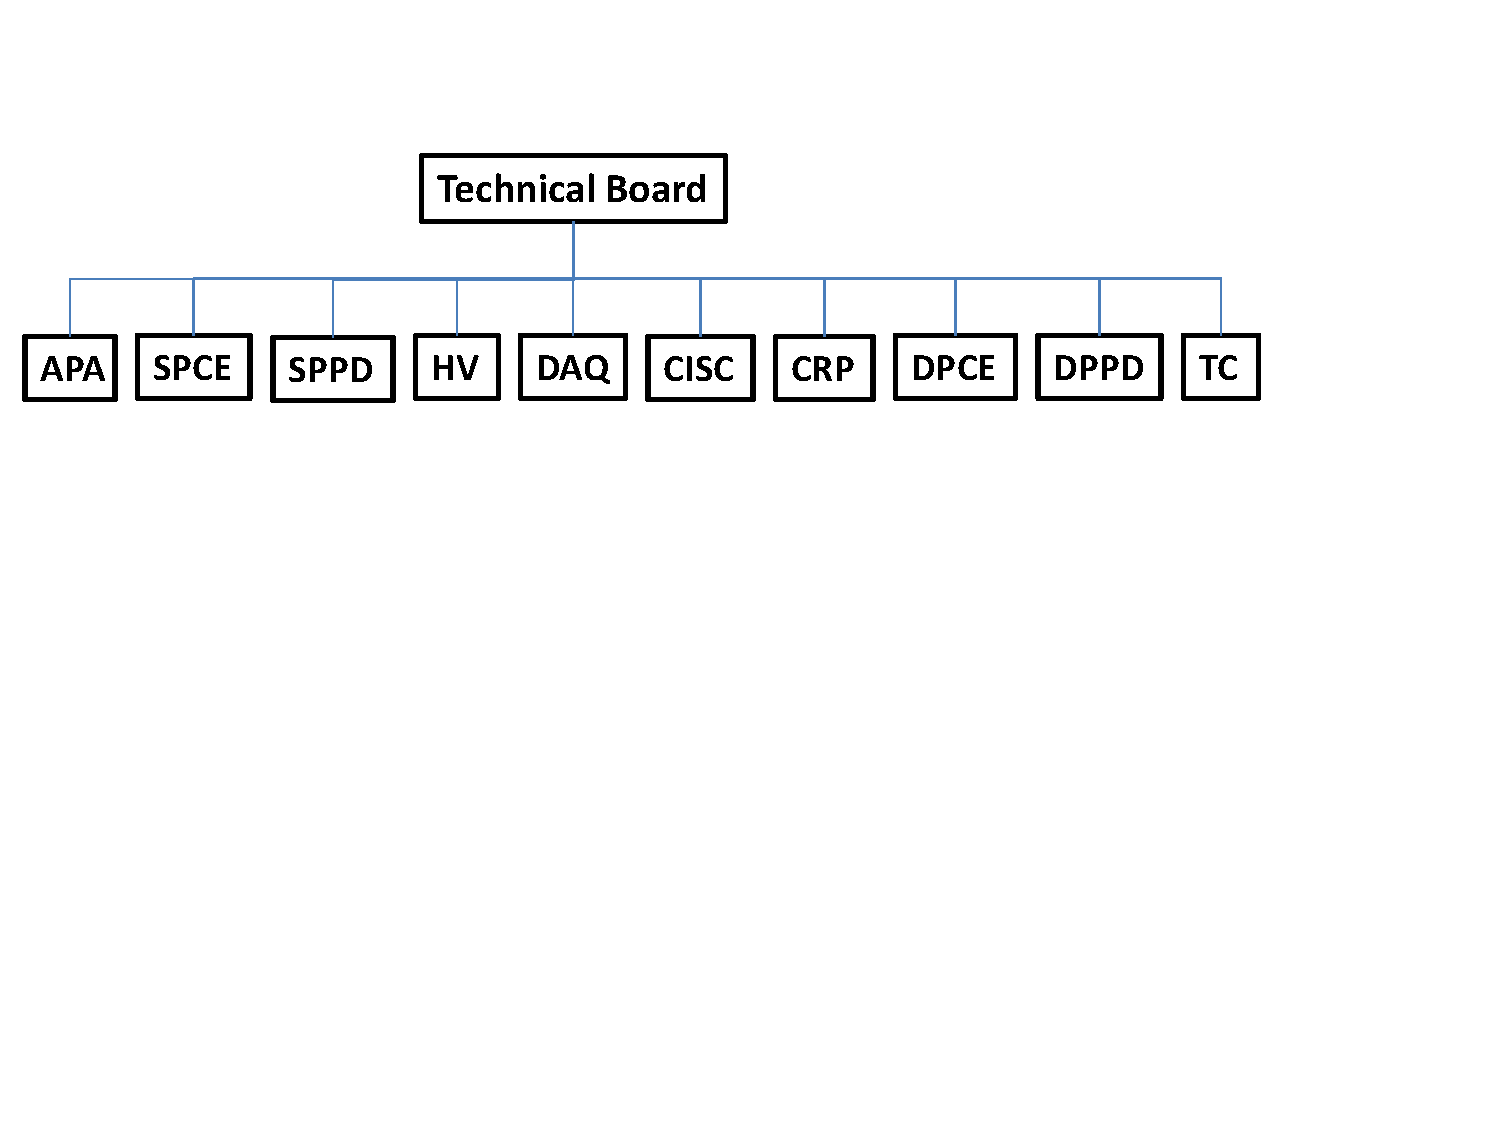
\includegraphics[width=0.8\textwidth]{far-detector-generic/figures/TB_Org_Chart}
    \caption{DUNE Technical Board.}
    \label{fig:TB_org}
  \end{center}
\end{figure}
It consists of all consortia scientific and technical leads. It meets
on a regular basis (approximately monthly) to review and resolve any
technical issues associated with the detector construction. It reports
through the EB to Collaboration Management. The
\dword{dune} Technical Board is chaired by the Technical
Coordinator. The DUNE collaboration management, including the EB is shown in
Fig.~\ref{fig:DUNE_org}.
\begin{figure}[htb]
  \begin{center}
    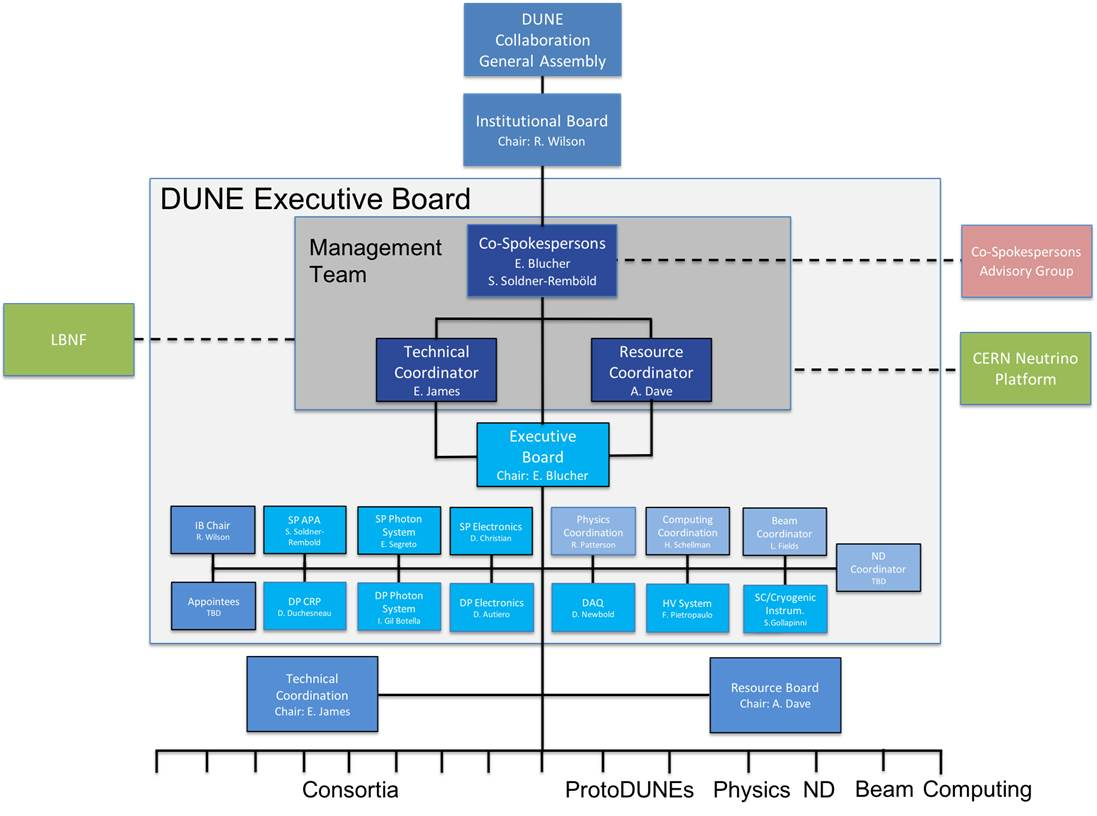
\includegraphics[width=0.8\textwidth]{far-detector-generic/figures/DUNE_mgmt}
    \caption{DUNE management organizational structure.}
    \label{fig:DUNE_org}
  \end{center}
\end{figure}



TC has several major project support tasks that need to be accomplished:
\begin{itemize}
  \item Assure that each consortia has a well defined and complete
    scope, that the interfaces between the consortia are sufficiently
    well defined and that any remaining scope can be covered by TC
    through Common Fund. Monitor the interfaces and consortia progress
    on delivering their scope.
  \item Develop an overall project schedule that includes reasonable
    production schedules from each consortia, testing plans and a well
    developed installation schedule. Monitor the overall schedule as
    well as the individual consortia schedules.
  \item Ensure that appropriate engineering and safety standards are
    developed and agreed to by all key stakeholders and that these
    standards are conveyed to and understood by each
    consortium. Monitor the design and engineering work.
  \item Ensure that all \dword{dune} requirements on \dword{lbnf} for
    conventional facilities, cryostat and cryogenics have been clearly
    defined and understood by each consortia. Monitor \dword{lbnf}
    progress on final conventional facility design.
  \item Ensure that all technical issues associated with scaling from
    \dword{protodune} have sufficient resources to converge on
    decisions that enable the detector to be fully integrated and
    installed.
  \item Ensure that the integration and QC processes for each
    consortia are fully developed and reviewed and that the
    requirements on an Integration and Test Facility are well defined.
\end{itemize}

Technical Coordination maintains a web page
(\url{https://web.fnal.gov/collaboration/DUNE/DUNE\%20Project/\_layouts/15/start.aspx\#/})
with links to project documents. TC maintains repositories of project
documents and drawings. These include the WBS, Schedule, risk
register, requirements, milestones, strategy, detector models and
drawings that define the \dword{dune} detector.


%%%%%%%%%%%%%%%%%%%%%%%%%%%%%%%%
\subsection{Schedule}
\label{sec:fdsp-coord-controls}

A series of tiered milestones are being developed for the \dword{dune}
project. The Tier-0 milestones are held by the Spokespersons and Host
Lab director. Three have been defined and the current target dates
are:
\begin{enumerate}
\item Start main cavern excavation \hspace{2.1in} 2019
\item Start detector \#1 installation \hspace{2.1in} 2022
\item Start operations of detector \#1--2 with beam \hspace{1in} 2026
\end{enumerate}
These dates will be revisited at the time of the TDR review.  Tier-1
milestones will be held by the Technical Coordinator and \dword{lbnf} Project
Manager and will be defined in advance of the TDR review. Tier-2
milestones will be held by the consortia.

A high level version of the \dword{dune} Project construction schedule
can be seen in Fig.~\ref{fig:DUNE_schedule}.
\begin{figure}[htb]
  \begin{center}
    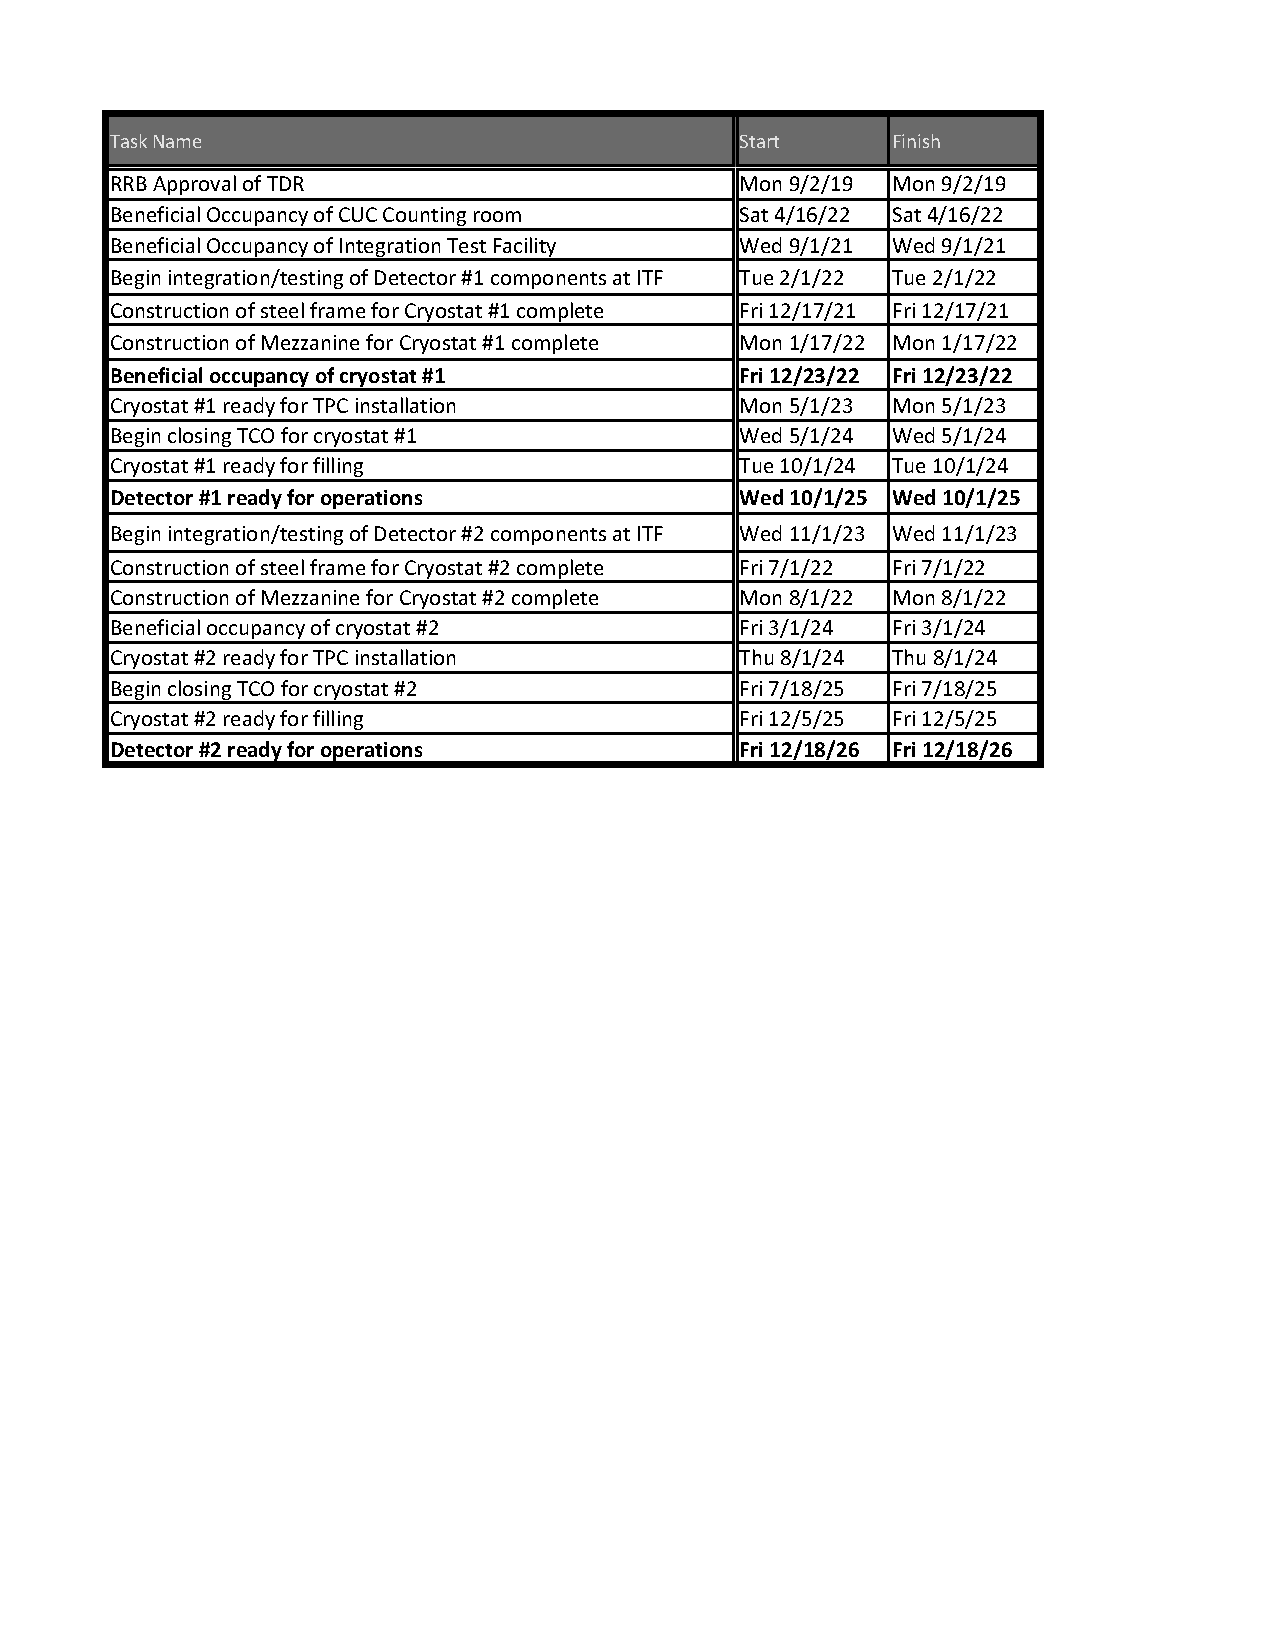
\includegraphics[width=0.8\textwidth]{far-detector-generic/figures/FD_Cnst_Schedule}
    \caption{Overall \dword{dune} Project Tier-1 milestones.}
    \label{fig:DUNE_schedule}
  \end{center}
\end{figure}
TC will maintain a master schedule that links all consortia schedules
and contains appropriate milestones to monitor progress. The master
schedule is envisioned to be maintained in MSProject as it is expected
that many consortia will use this tool. It is currently envisioned as
three levels of control and notification milestones. The highest level
containing external milestones, with the second level containing the
key milestones for TC to monitor deliverables and installation
progress, and the third level containing the inter-consortia
links. The master schedule will go under change control after
agreement with each consortium on the notification milestone dates and
the TDR is approved.

A schedule of key consortia activity in the period 2018--19 leading up
to the TDR has been developed.

In order to ensure that the \dword{dune} detector remains on schedule, TC
will monitor schedule statusing from each consortium, will organize
reviews of schedules and risks as appropriate.

A monthly report with input from all consortia will be published by
TC. This will include updates on consortia technical progress and
updates from TC itself.


%%%%%%%%%%%%%%%%%%%%%%%%%%%%%%%%
\subsection{Risk}
\label{sec:fdsp-coord-risk}

The successful operation of \dword{protodune} will retire a great many
potential risks to \dword{dune}. This includes most risks associated with the
technical design, production processes, quality assurance, integration
and installation. Residual risks remain relating to design and
production modifications associated with scaling to \dword{dune}, mitigations
to known installation and performance issues in \dword{protodune}, underground
installation at SURF and organizational growth.

[Enumerate remaining technical risks?.... or all risks?.... 600kV, HV
  in general, noise, dead channels, 20 year operation, QC in general,
  ADC/coldata, photon light yield, purity, LAr surface stbility, LEM
  gain, dual-phase LAr surface cleanliness, cathode/FC discharge to
  cryostat, incomplete calibration plan, incomplete connection of
  design to physics; funding, production schedule, integration plan,
  testing, underground installation, ...]

Key risks for TC to manage include the following:
\begin{enumerate}
    \item Too much scope is unaccounted for by the consortia and falls
      to TC and Common Fund.
    \item Insufficient organizational systems are put into place to
      ensure that this complex international mega-science project,
      including TC, FNAL as Host Lab, SURF, DOE and all international
      partners continue to successfully work together to ensure
      appropriate rules and services are provided to enable success of
      the project.
  \item TC is unable to obtain sufficient personnel resources so as to
    be able to ensure that TC can oversee and coordinate all of its
    project tasks.  While the US has a special responsibility towards
    TC as host country, it is expected that personnel resources will
    be directed to TC from each collaborating country. Related to this
    risk is the fact that consortia deliverables are not really
    stand-alone subsystems; they are all parts of a single TPC. This
    elevates the requirements on coordination between consortia.
\end{enumerate}

The consortia have provided preliminary versions of risk analyses that
have been collected on the TC webpage. These are being developed into
an overall risk register that will be monitored and maintained by TC
in coordination with the consortia.

%%%%%%%%%%%%%%%%%%%%%%%%%%%%%%%%
\subsection{Reviews}
\label{sec:fdsp-coord-reviews}

Technical Coordination is responsible to review all stages of detector
development and works with each consortium to arrange reviews of the
design, production readiness, production progress and operational
readiness of their system.  These reviews provide input for the TB to
make technical decisions.  Review reports are tracked by TC and
provide guidance as to key issues that will require engineering
oversight by the TC integration engineering team. TC will maintain a
calendar of \dword{dune} reviews.

TC will work with consortia leaders to review all detector designs,
with an expectation for a preliminary design review, followed by a
final design review. All major technology decisions will be reviewed
prior to down-select.

Start of production of DUNE detector elements can commence only after
successful production readiness review. Regular production progress
reviews will be held once production has commenced.

%%%%%%%%%%%%%%%%%%%%%%%%%%%%%%%%
\subsection{Quality Assurance}
\label{sec:fdsp-coord-qa}


The \dword{lbnf}/\dword{dune} Quality Assurance Plan outlines the QA
requirements for all \dword{dune} consortia and describes how the
requirements shall be met. The consortia will be responsible for
implementing a quality plan that meet the requirements of the
\dword{lbnf}/\dword{dune} Quality Assurance Plan.  The consortia
implement the plan through the development of individual quality
plans, procedures, guides, QC inspection and test requirements and
travelers/test reports.  In lieu of a consortia Specific Quality Plan,
the consortia may work under the \dword{lbnf}/\dword{dune} Quality
Assurance Plan and develop Manufacturing/QC Plans, procedures and
documentation specific to their work scope.  The \dword{dune}
Technical Coordinator and consortia Leaders are responsible for
providing the resources needed to conduct the Project successfully,
including those required to manage, perform and verify work that
affects quality.  The \dword{dune} consortia Leaders are responsible
for identifying adequate resources to complete the work scope and to
ensure that their team members are adequately trained and qualified to
perform their assigned work.

The consortia work will be documented on travelers and applicable test
or inspection reports. Records of the fabrication, inspection and
testing will be maintained. When a component has been identified as
being in noncompliance to the design, the nonconforming condition
shall be documented, evaluated and dispositioned as use-as-is (does
not meet design but can meet functionality as is), rework (bring into
compliance with design), repair (will be brought into meeting
functionality but will not meet design) and scrap.

The \dword{lbnf}/\dword{dune} Quality Assurance Manager (QAM) reports
to the \dword{lbnf} Project Manager and \dword{dune} Technical
Coordinator and provides oversight and support to the consortia
Leaders to ensure a consistent quality program.
\begin{enumerate}
  \item The QAM will plan reviews as independent assessments to assist
    the \dword{dune} Technical Coordinator in identifying opportunities for
    quality/performance-based improvement and to ensure compliance
    with specified requirements.
  \item The QAM is responsible to work with the consortia in
    developing their QA/QC Plans.
  \item The QAM will review consortia QA/QC activity, including
    production site visits.
  \item The QAM will participate in consortia Design Reviews, conduct
    Production Readiness Reviews prior to the start of production,
    conduct Production Progress Reviews on a regular basis (as
    described in Section~\ref{sec:fdsp-coord-reviews}, and perform
    follow-up visits to consortia facilities prior to shipment of
    components to ensure all components and documentation are
    satisfactory.
\item The QAM is responsible for performing assessments at the
  Integration Facility, the Far Site and the Near Site to
  ensure the activities performed at these locations are in accordance
  with the \dword{lbnf}/\dword{dune} QA Program and applicable procedures,
  specifications and drawings.
\end{enumerate}

%%%%%%%%%%%%%%%%%%%%%%%%%%%%%%%%
\subsubsection{Document Control}
\label{sec:fdsp-coord-document}

TC maintains repositories of project documents and drawings in two
document management systems.  DUNE Project documents will be stored in
the DUNE DocDB (\url{https://docs.dunescience.org}). DUNE drawings
will be stored in EDMS
(\url{https://edms.cern.ch/ui/#!master/navigator/project?P:1637280201:1637280201:subDocs}).
TC will maintain approved versions of QA, QC and testing plans,
installation plans, engineering and safety standards in the DUNE
DocDB.

Consortia have developed initial interface documents that will be put
under change control and managed by the TC integration engineering
team along with the consortia involved. These are currently in DocDB
and will likely go under change control later in 2018, although they
will continue to be developed through the TDR.


%%%%%%%%%%%%%%%%%%%%%%%%%%%%%%%%
\subsection{ES\&H}
\label{sec:fdsp-coord-esh}

The \dword{dune} Environmental, Safety and Health (ESH) program is
described in the \dword{lbnf}/\dword{dune} Integrated Environmental,
Safety and Health Plan. This plan is maintained by the
\dword{lbnf}/\dword{dune} ESH Manager, who reports to the \dword{lbnf}
Project Manager and the TC. The ESH is responsible to work with the
consortia in reviewing their hazards and their ESH plans.  The ESH
Manager is responsible to review ESH at production sites, integration
sites and at SURF. It is expected that the ESH reviews will be
conducted as part of the PRR and PPR process described in
Section~\ref{sec:fdsp-coord-reviews}.
